\chapter{Cahier des charges}

\section{Introduction}

Le but de ce projet est de réaliser un télescope électronique. C'est-à-dire un télescope doté d'une caméra et dont les mouvements sont pilotables via une interface homme-machine.

\vspace{1cm}

Ce projet se base sur un projet existant~: Un télescope de type Newton conçu pour être imprimable à l'imprimante 3D. (Le projet semble avoir récemment disparu d'internet).

Lien du projet~: {\href{https://blog.dagoma.fr/telescope-imprime-en-3d/}{\codeinline{text}{https://blog.dagoma.fr/telescope-imprime-en-3d/}}}

\begin{figure}[H]
	\centering
    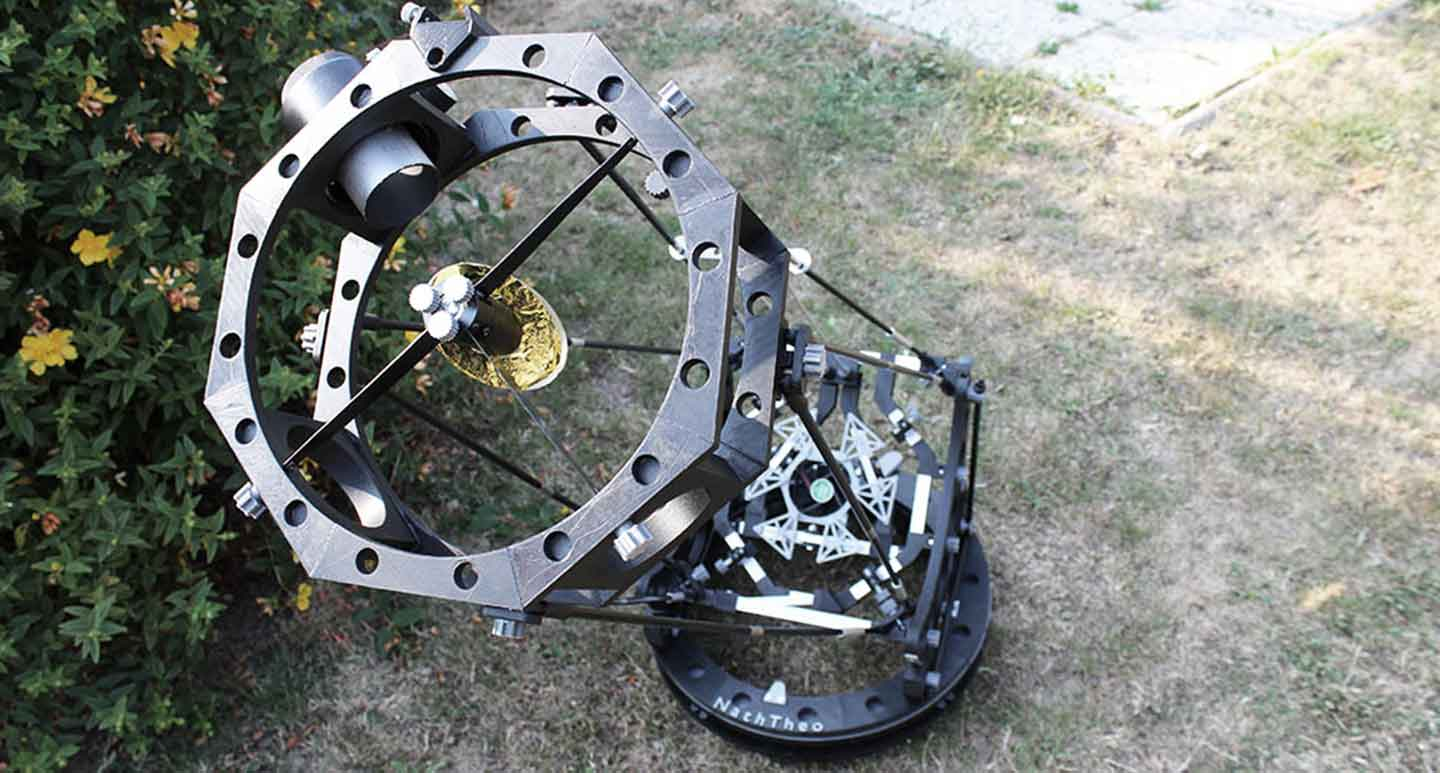
\includegraphics[width=0.9\linewidth]{\figures/photo_telescope.jpg}
    \decoRule
    \caption[
    Photo du télescope imprimé]{
    Photo du télescope imprimé}
    \label{fig:Photo du télescope imprimé}
	\end{figure}

\vspace{1cm}

Concernant la politique du projet, nous le souhaitons libre et accessible. C'est pourquoi il sera disponible sur internet sous licence de type copyleft (GPL) et nous travaillerons avec des outils de production libres également, que quiconque peut utiliser.

\section{Nécessité du traçage d'astre}

Le traçage d'astre, vu au départ comme une fonctionnalité intéressante, s'est imposé comme une fonctionnalité nécessaire sur laquelle repose beaucoup de l'intérêt que porte le projet. En effet il peut être particulièrement difficile pour une personne non initiée à l'astronomie de positionner le télescope vers un astre précis ou de reconnaître un astre que l'on observe. Il nous est donc apparu primordial que le télescope permette d'affranchir l'utilisateur de la nécessité d'avoir des bases en astronomie pour observer le ciel.

\vspace{1cm}

En étudiant les solutions disponibles nous avons trouvé des logiciels de simulation du ciel, comme par exemple le logiciel libre Stellarium.

\begin{figure}[H]
    \centering
    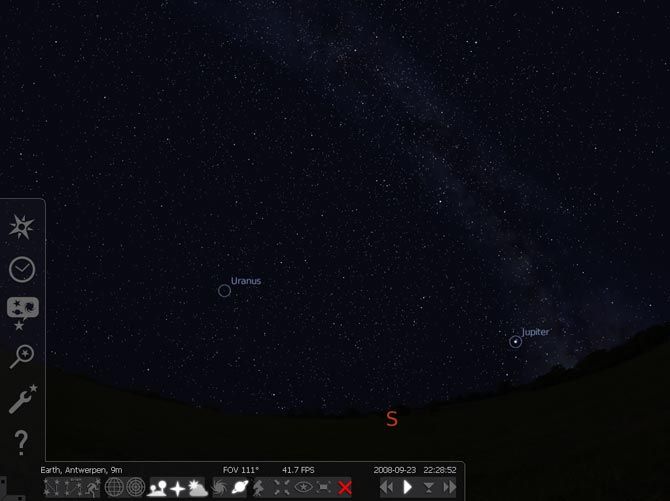
\includegraphics[width=0.49\linewidth]{\figures/photo_stellarium_1.jpg}
	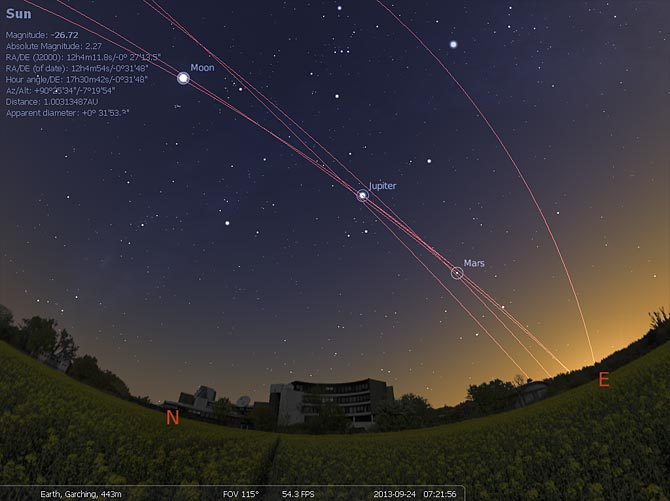
\includegraphics[width=0.49\linewidth]{\figures/photo_stellarium_2.jpg}
    \decoRule
    \caption[
    Captures d'écran de Stellarium]{
    Captures d'écran de Stellarium}
    \label{fig:Captures d'écran de Stellarium}
    \end{figure}

\vspace{1cm}

Celui-ci permet notamment~:
\begin{itemize}[label=$\bullet$]
	\item De connaître les coordonnées d'un astre par rapport à l'endroit sur terre où se situe l'observateur.
	\item De s'orienter dans le ciel selon des coordonnées.
	\item De s'interfacer avec d'autres systèmes logiciels et/ou matériels
	\end{itemize}

Nous avons donc décidé dans un premier temps de développer une interface pour piloter le télescope depuis un ordinateur distant doté de Stellarium. Puis éventuellement d'embarquer Stellarium dans l'ordinateur du télescope. Ainsi Stellarium fera partie intégrante de son interface utilisateur.

Celle-ci pourrait être alors un menu discret permettant de passer de l'exploration virtuelle du ciel à la vue correspondante à travers le télescope à d'autres élément comme un dispositif d'amélioration de la qualité des images prises.

\section{Nécessité d'une centrale inertielle et d'un GPS}

L'utilisation d'un logiciel de traçage d'astre tel Stellarium nécessite la compatibilité du télescope avec les coordonnées d'azimut et d'élévation couramment utilisées en astronomie. Il est également nécessaire pour cela de savoir de quel endroit sur terre le télescope observe le ciel, d'où l'utilisation d'un GPS.

\vspace{1cm}

Pour connaître l'azimut et l'élévation, il faut avoir des repère dans les deux dimensions. Un magnétomètre permet de déterminer la direction du nord et un accéléromètre permet de connaître la direction du sol, c'est à dire la verticale.

Une centrale inertielle est un composant intégrant un magnétomètre, un accéléromètre et un gyroscope. Elle permet de connaître directement les coordonnées absolues de son orientation dans l'espace.

\section{Aperçu d'un logiciel de traitement d'images en astronomie}

Le traitement d'images en astronomie est un domaine particulier de la retouche photo puisqu'il ne s'agit pas simplement de créer de jolies choses mais de faire ressortir certaines choses d'une image ou d'une série d'images. Il s'agit donc de garder une pertinence physique lors des retouches.

Certains logiciels sont spécialisés dans le traitement d'images du ciel. Parmi les logiciels libres Siril semble être l'un des plus aboutis. Il dispose de nombreux outils et permet de faire de nombreux types de retouches. Un atout intéressant est qu'il permet d'utiliser des scripts pour traiter des images.

\begin{figure}[H]
	\centering
    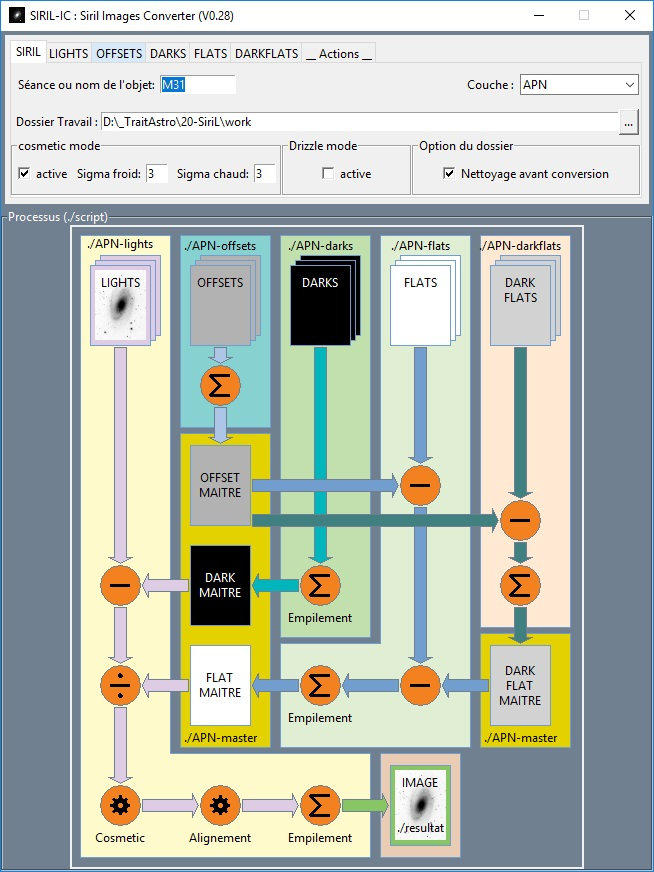
\includegraphics[height=0.3\linewidth]{\figures/photo_siril1.jpg}
    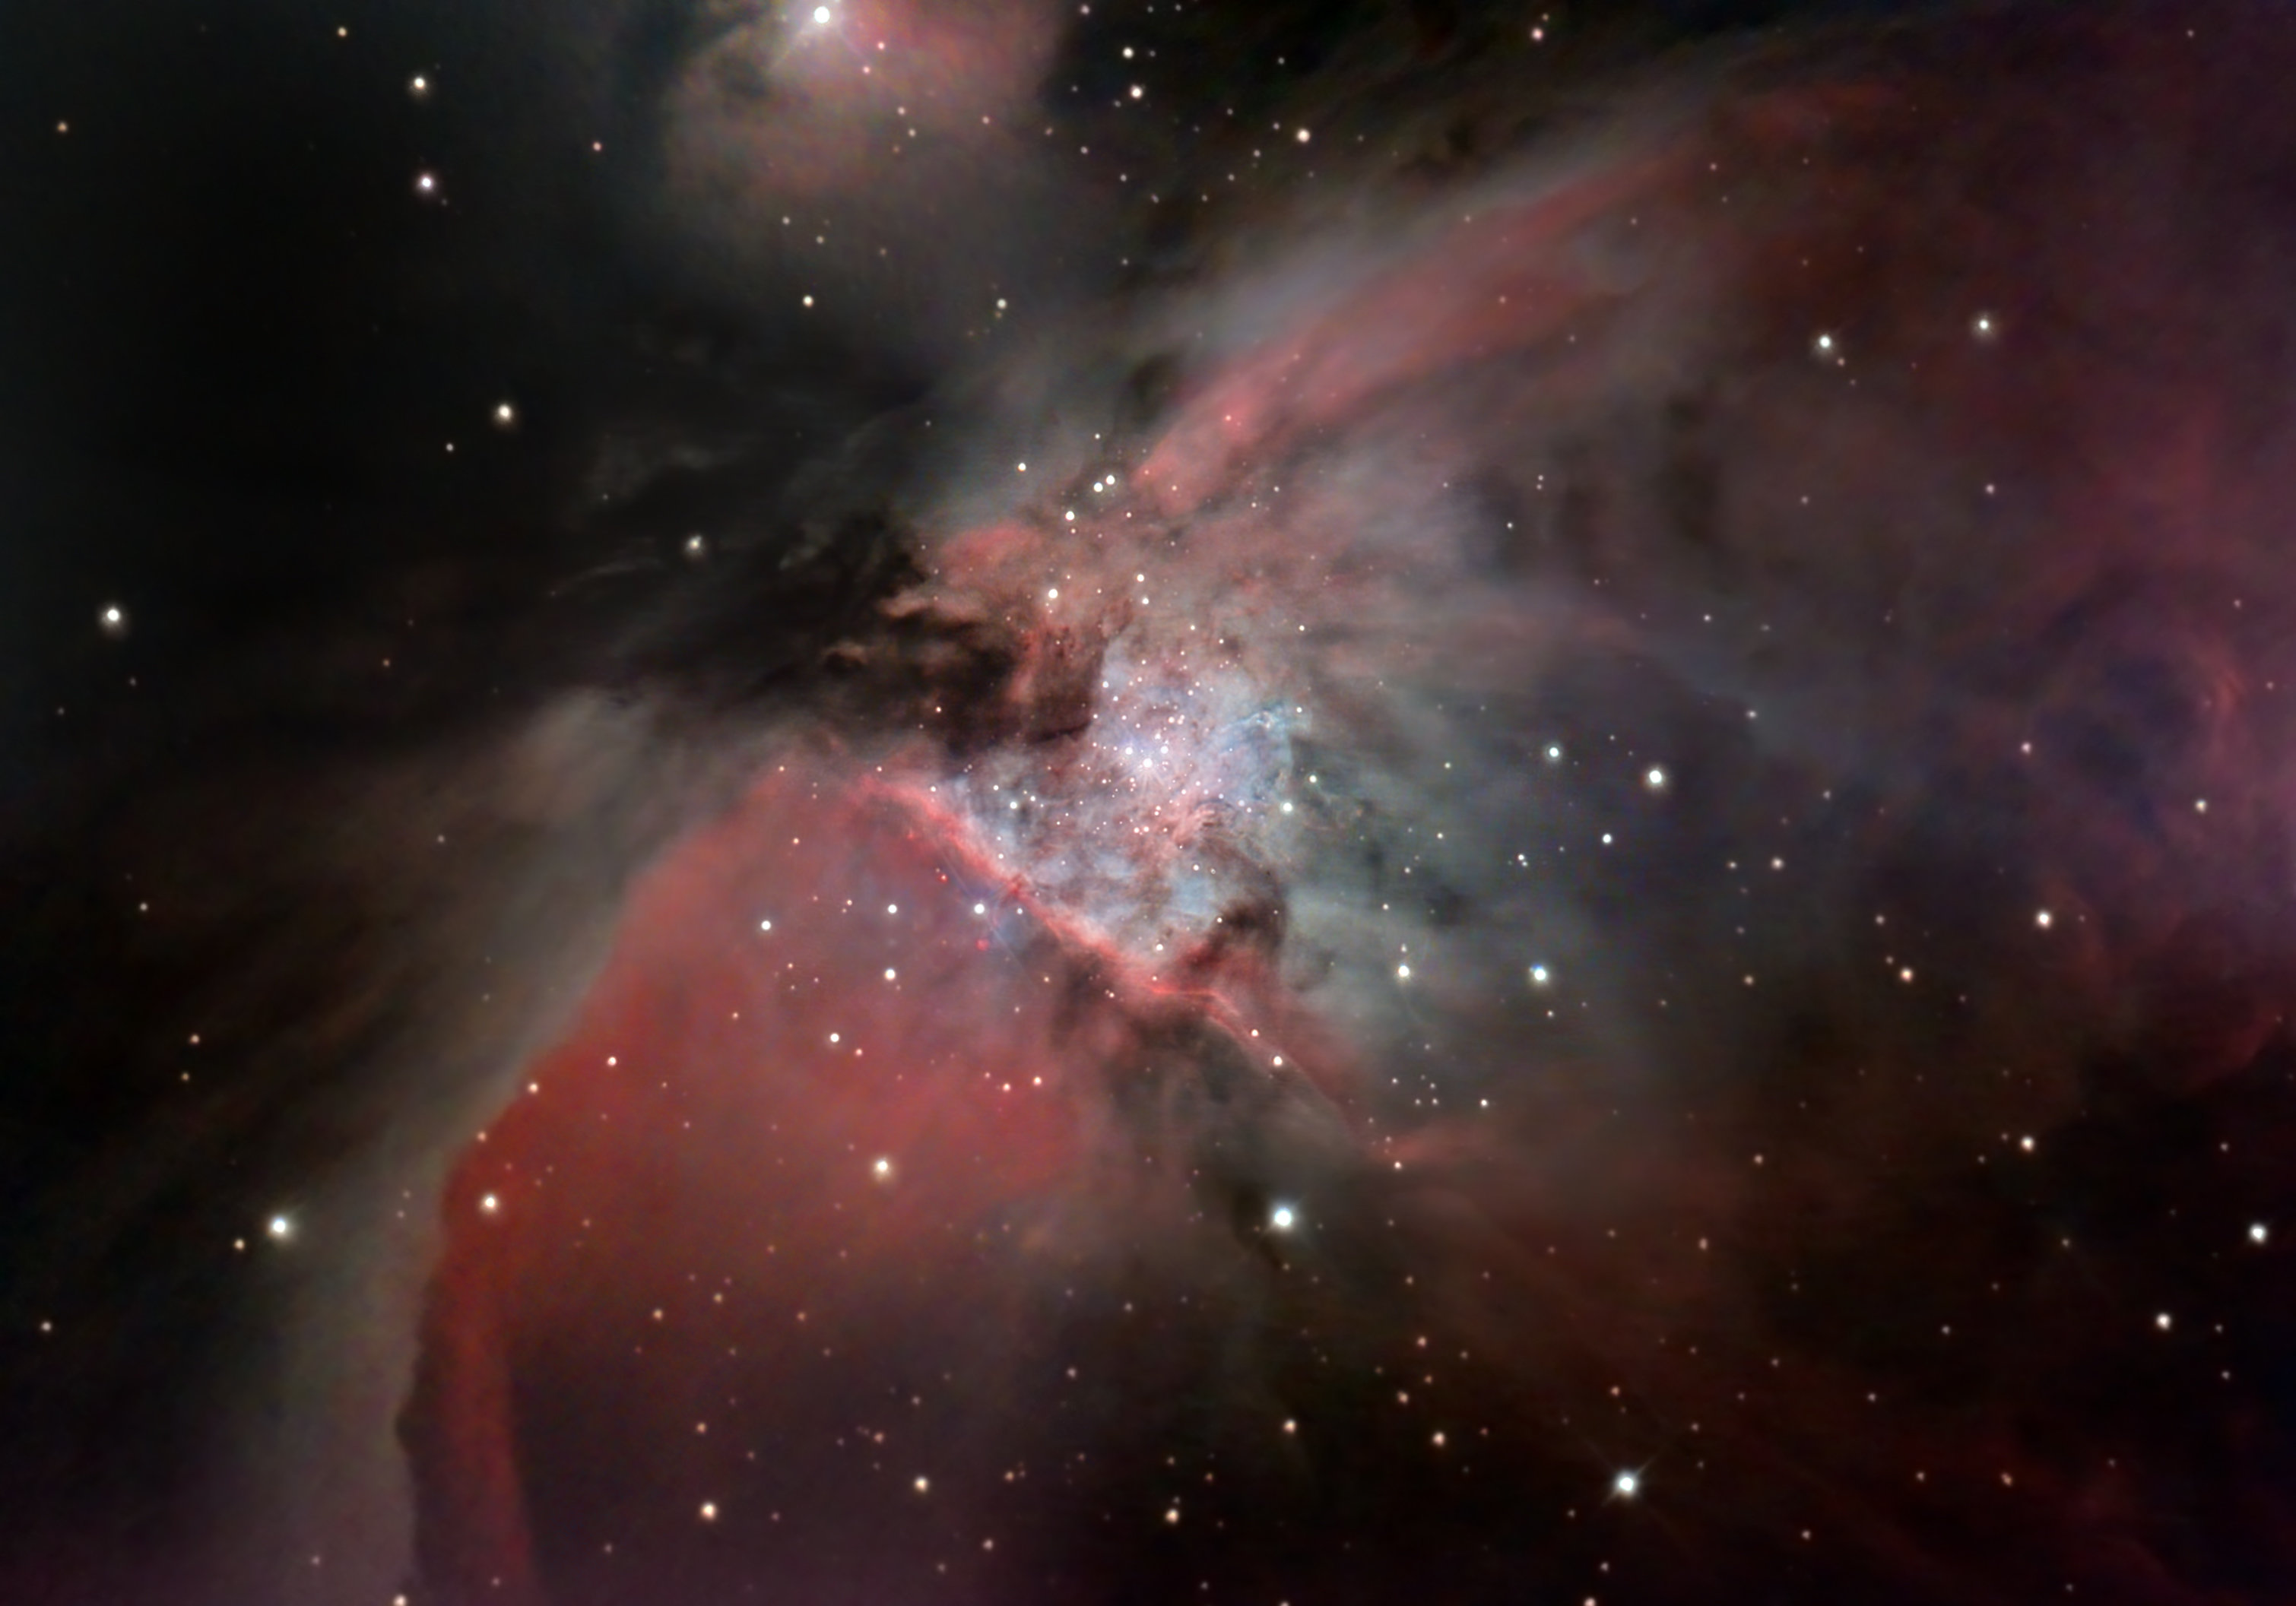
\includegraphics[height=0.3\linewidth]{\figures/photo_siril7.jpg}
    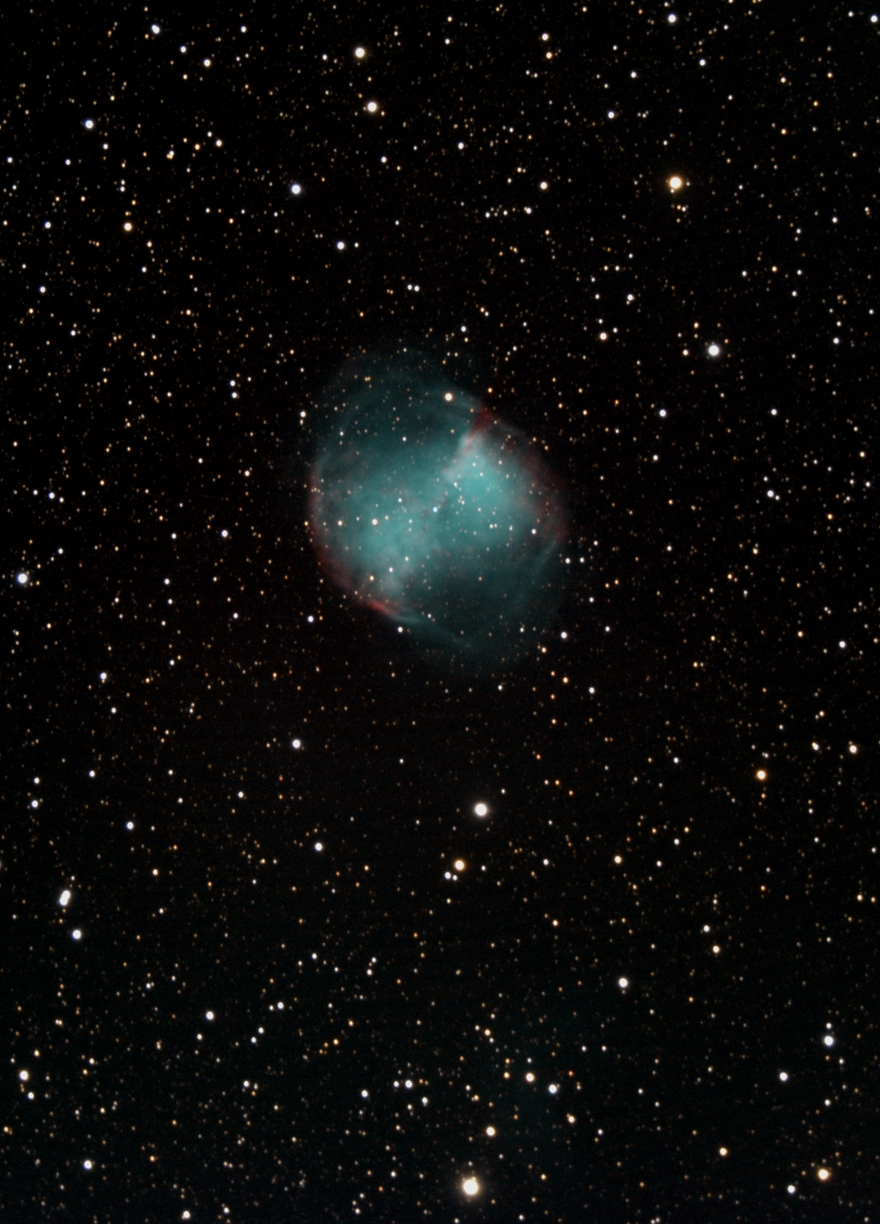
\includegraphics[height=0.3\linewidth]{\figures/photo_siril5.jpg}
    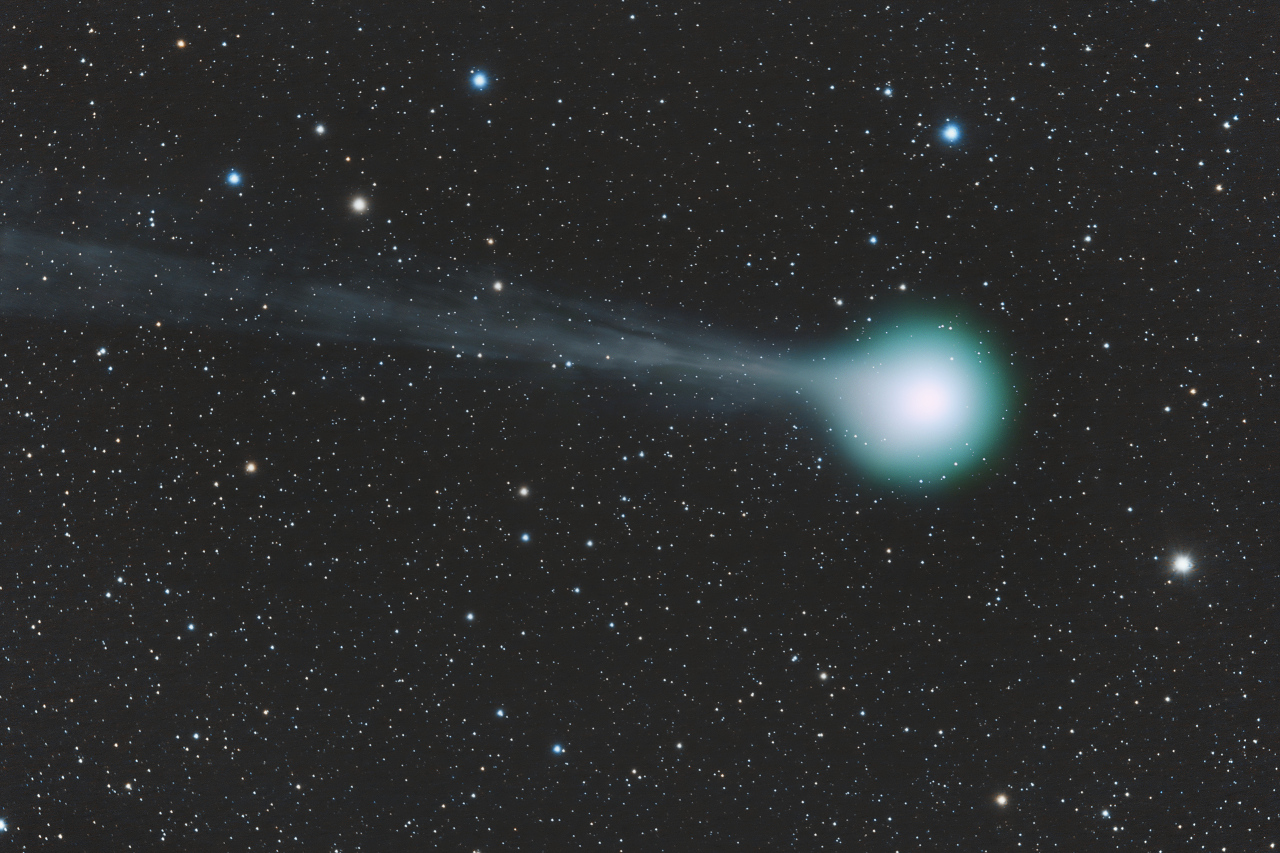
\includegraphics[height=0.3\linewidth]{\figures/photo_siril2.jpg}
    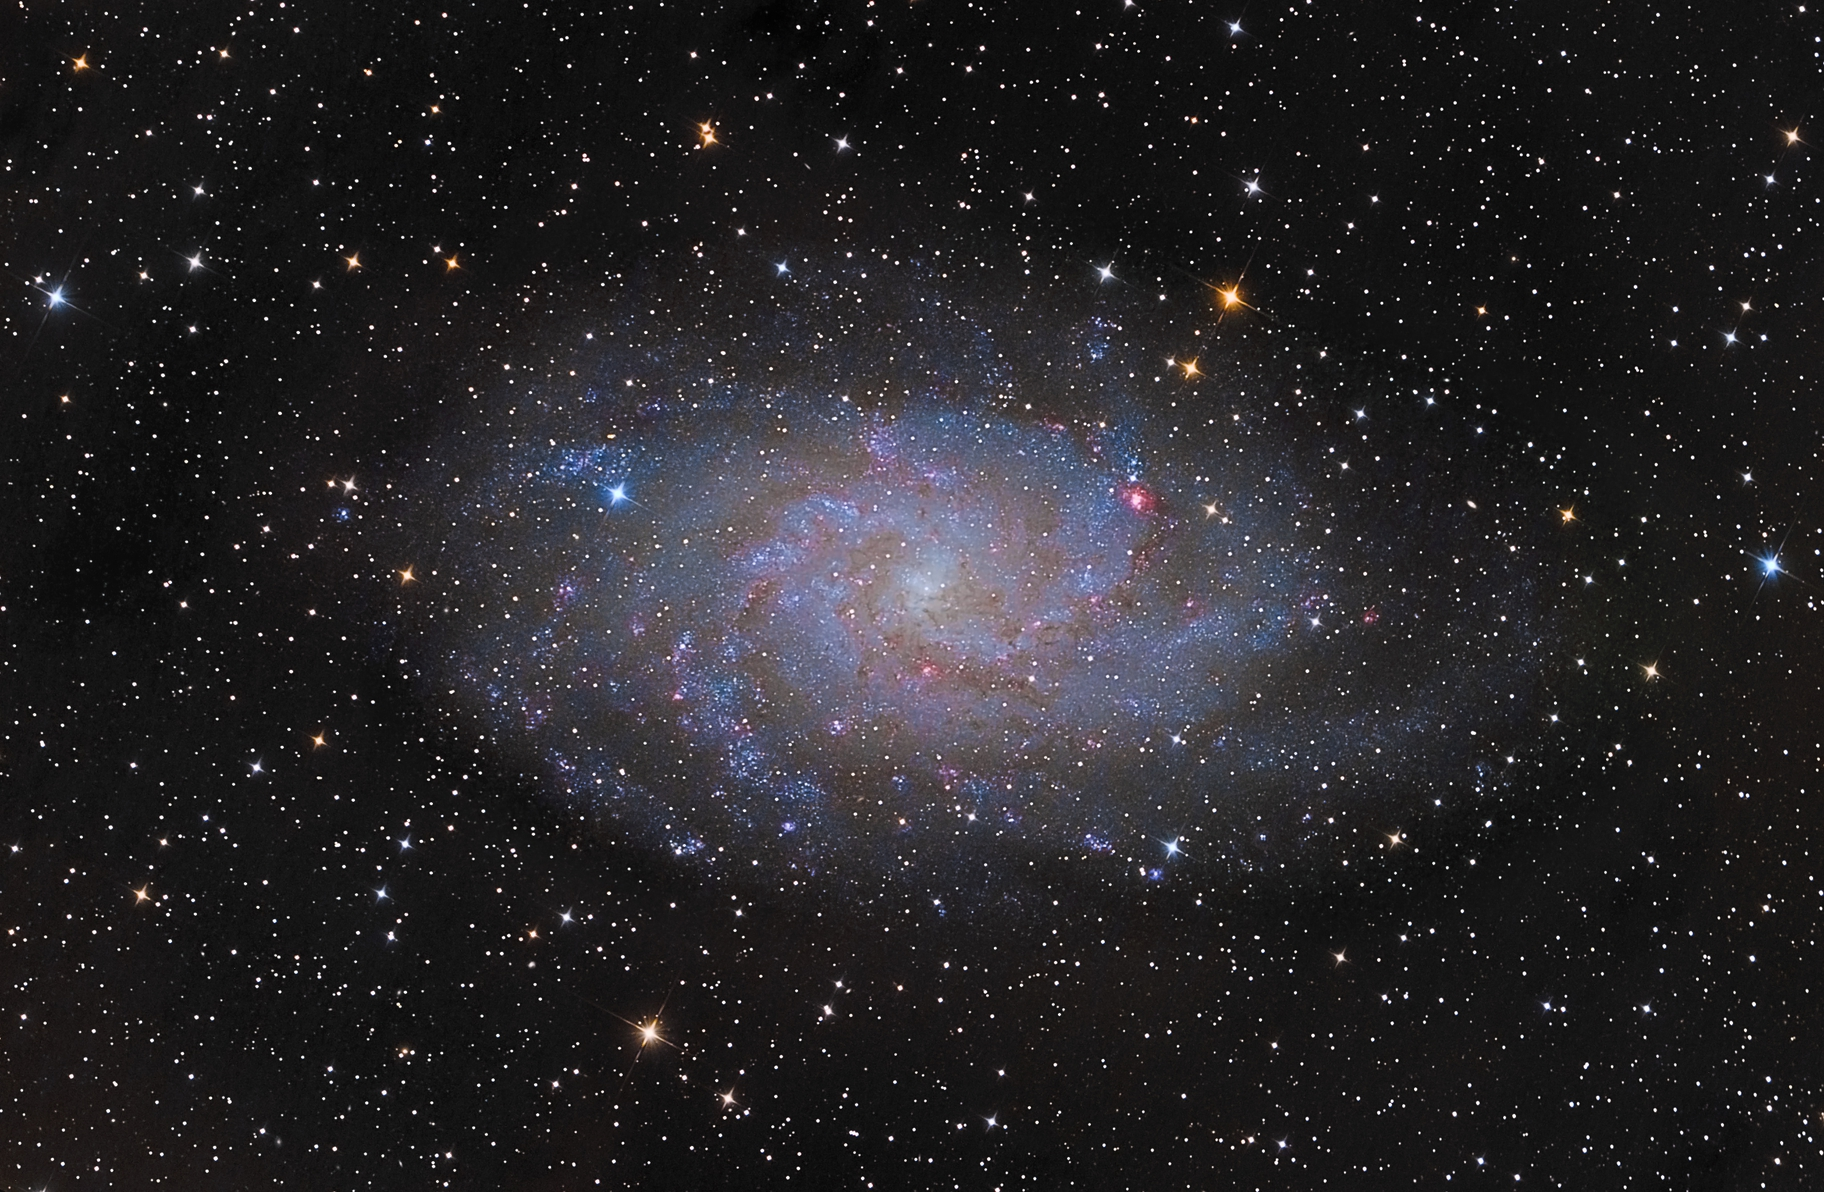
\includegraphics[height=0.3\linewidth]{\figures/photo_siril3.jpg}
    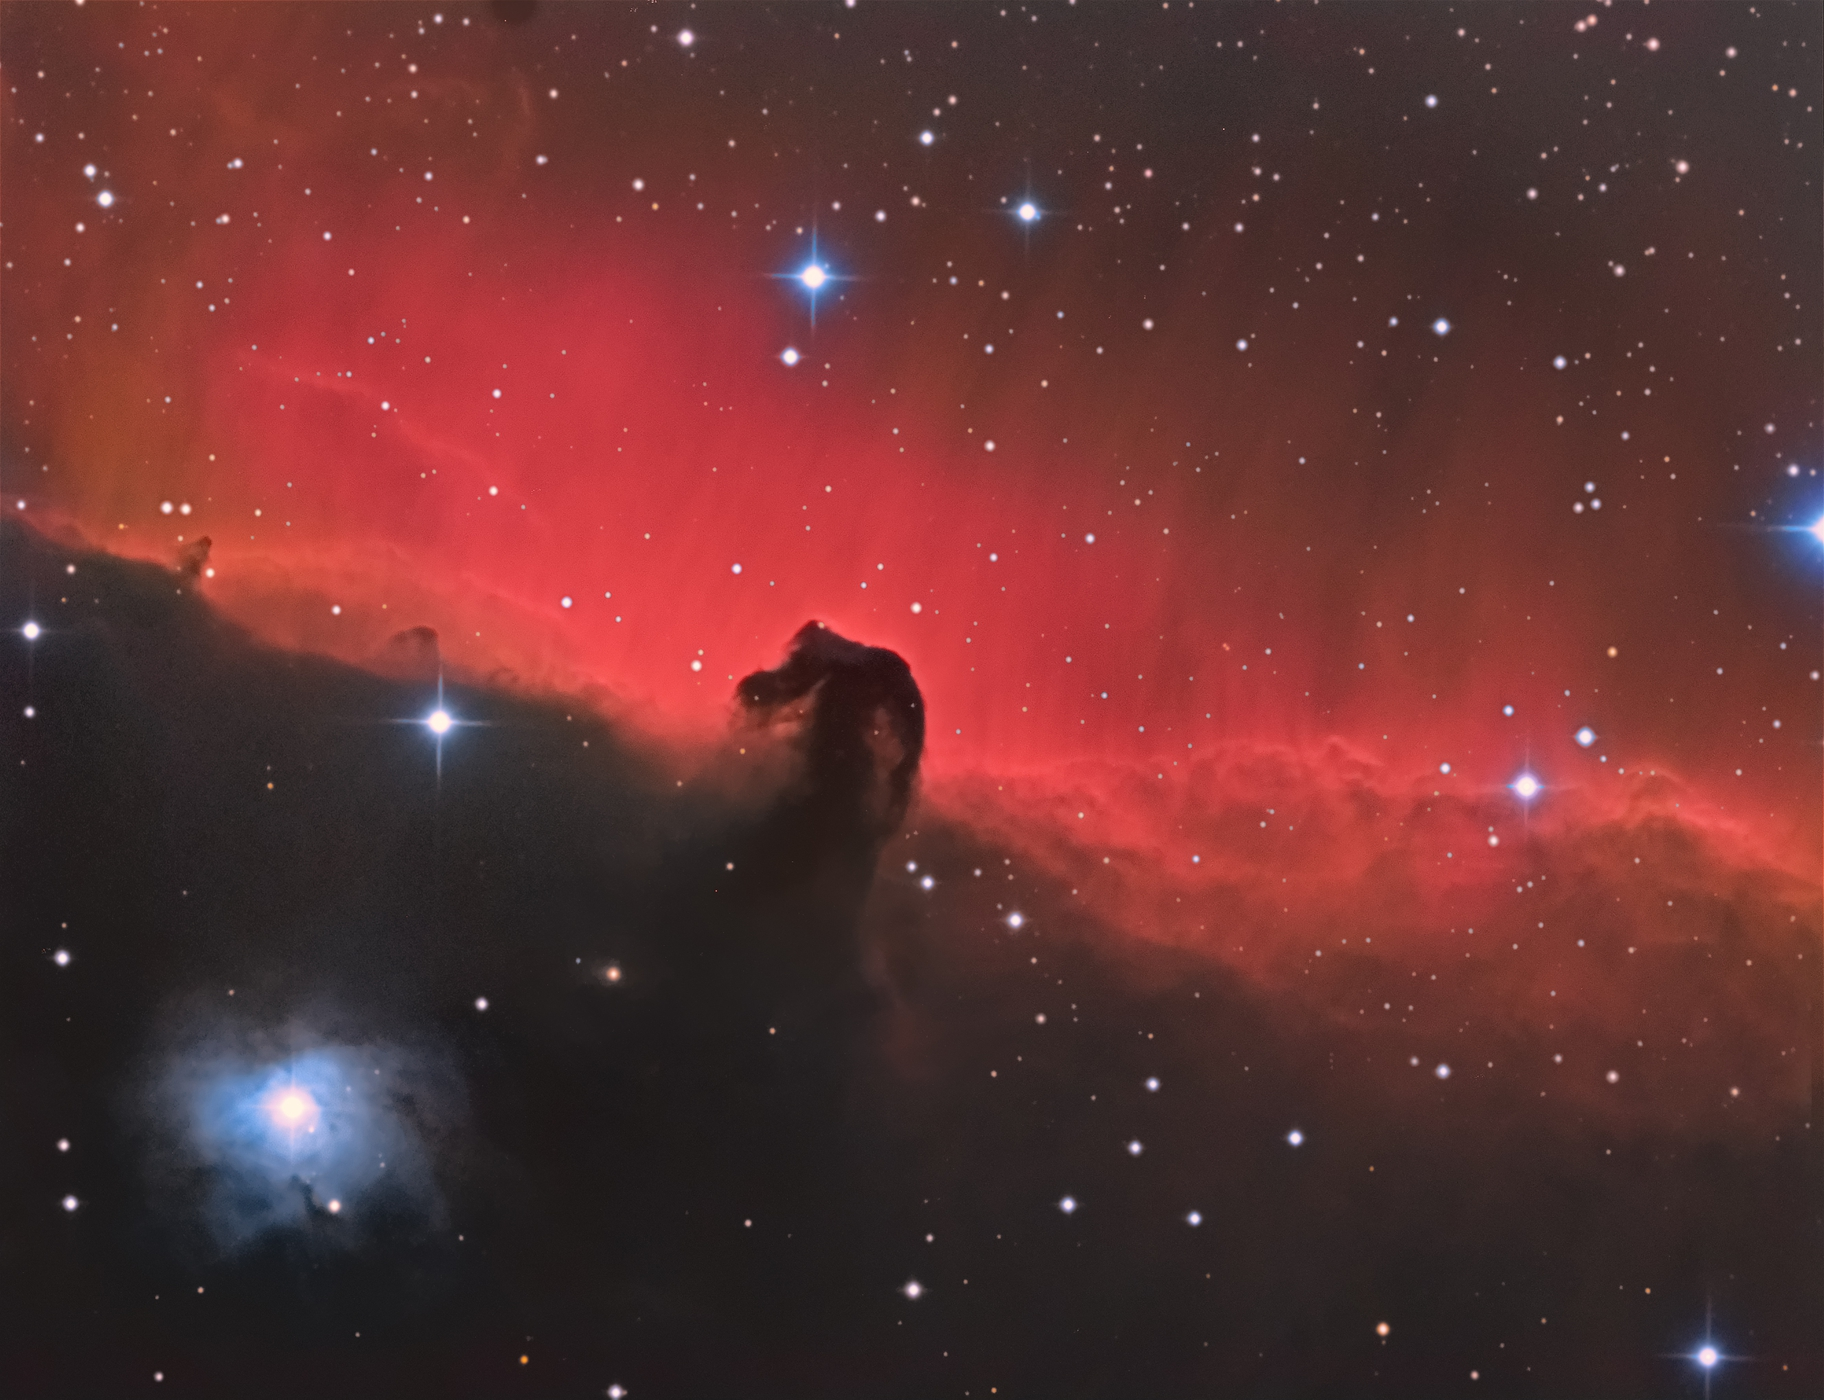
\includegraphics[height=0.3\linewidth]{\figures/photo_siril4.jpg}
    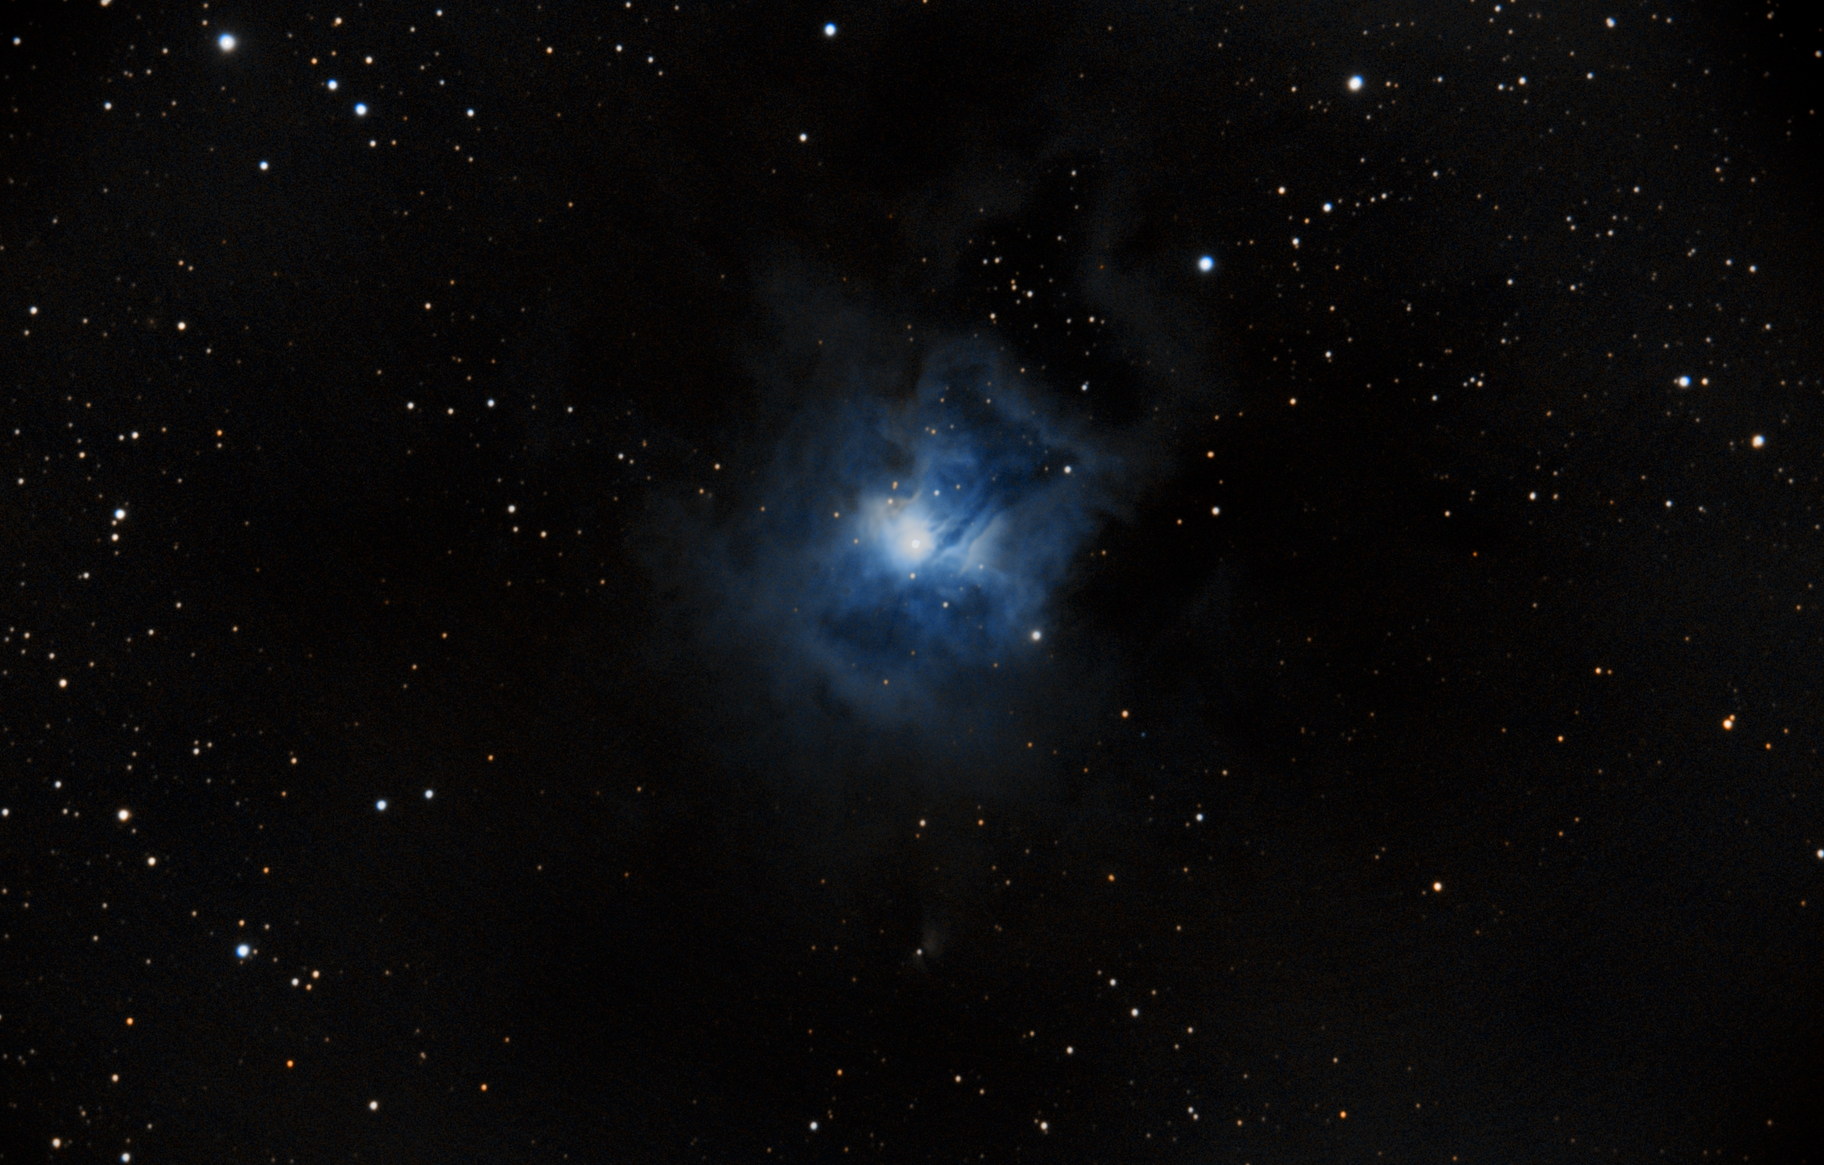
\includegraphics[height=0.3\linewidth]{\figures/photo_siril6.jpg}
    \decoRule
    \caption[
    Aperçu de Siril et de quelques clichés améliorés par son utilisation]{
    Aperçu de Siril et de quelques clichés améliorés par son utilisation}
    \label{fig:Aperçu de Siril et de quelques clichés améliorés par son utilisation}
	\end{figure}

\section{Spécifications techniques}

Certaines fonctionnalités devront impérativement être implémentées pour que le télescope soit validé. D'autres sont envisagées et seront implémentées dans la mesure du possible avant l'évaluation de ce projet. Certaines le seront éventuellement passé cette date, d'autres ne le seront peut être jamais.

De plus nous nous imposons dès le départ l'utilisations de certains matériels.

\subsection{Fonctionnalités obligatoires}

Le télescope devra être capable d'effectuer des mouvements d'azimut à 360\textdegree et des mouvements d'élévation dont l'amplitude dépend de la structure du télescope utilisé comme point de départ.

\vspace{1cm}

Il disposera d'une caméra permettant de prendre des clichés.

\vspace{1cm}

Pouvoir suivre les astres et se positionner dans le ciel est une fonctionnalité primordiale, elle devra être implémentée en priorité. De fait Stellarium jouera un rôle central dans l'interface utilisateur du télescope. Une solution où un ordinateur distant équipé de Stellarium pilote le télescope sera d'abord développée.

\vspace{1cm}

Idéalement le télescope devrait être accessible à un ordinateur par Wifi.

%Concernant l'interface homme-machine, il disposera d'une interface réseau rudimentaire ainsi que d'un écran tactile. Il sera donc doté d'un logiciel de pilotage.

\subsection{Fonctionnalités envisagées}

Une seconde interface utilisateur où Stellarium serait embarqué dans le télescope qui disposerait d'un écran tactile est envisagée. Ainsi le télescope se suffirait à lui même.

Il existe également une version de Stellarium disponible pour smartphone, il devient donc envisageable de piloter le télescope avec un téléphone. La version Android pourrait d'ailleurs être une piste à explorer pour embarquer ce logiciel.
 
\vspace{1cm}

L'ajout d'une fonctionnalité permettant d'améliorer la qualité des images de façon automatique ou simplifié serait intéressant. Siril semble être une direction prometteuse à ce sujet.

Le traitement des photos est une fonctionnalité n'ayant de sens que si le télescope fonctionne pleinement, cette fonctionnalité ne peut donc être prioritaire.

\vspace{1cm}

L'ajout d'une batterie permettant l'autonomie du télescope est également envisagé mais n'est pas vu comme une priorité.

\vspace{1cm}

Une solution de zoom optique pourrait également être intéressante s'il n'est pas trop compliqué ou onéreux d'en mettre une en place. La valeur ajoutée de cette fonctionnalité serait assez grande puisqu'elle permettrait de rendre le télescope polyvalent quant à ce qu'il est capable d'observer.

\subsection{Matériel}

Nous avons choisi d'utiliser comme élément central un SoC (System on Chip) Raspberry-Pi qui, en dépit de ses faibles capacités d'industrialisations, a l'avantage d'être populaire dans le milieu de l'électronique amateur, c'est-à-dire le publique le plus susceptible d'être intéressé par ce genre de projet.

Nous avons au départ envisagé l'usage d'une carte PICO-PI-IMX7D de NXP pour nous familiariser à un environnement de travail plus professionnel, que nous avons ensuite délaissé dans l'optique d'embarquer Stellarium dans le télescope. En effet la carte PICO-IMX7D ne dispose ni du GPU de la Raspberry-Pi, ni de suffisamment de RAM.

\begin{figure}[H]
    \centering
    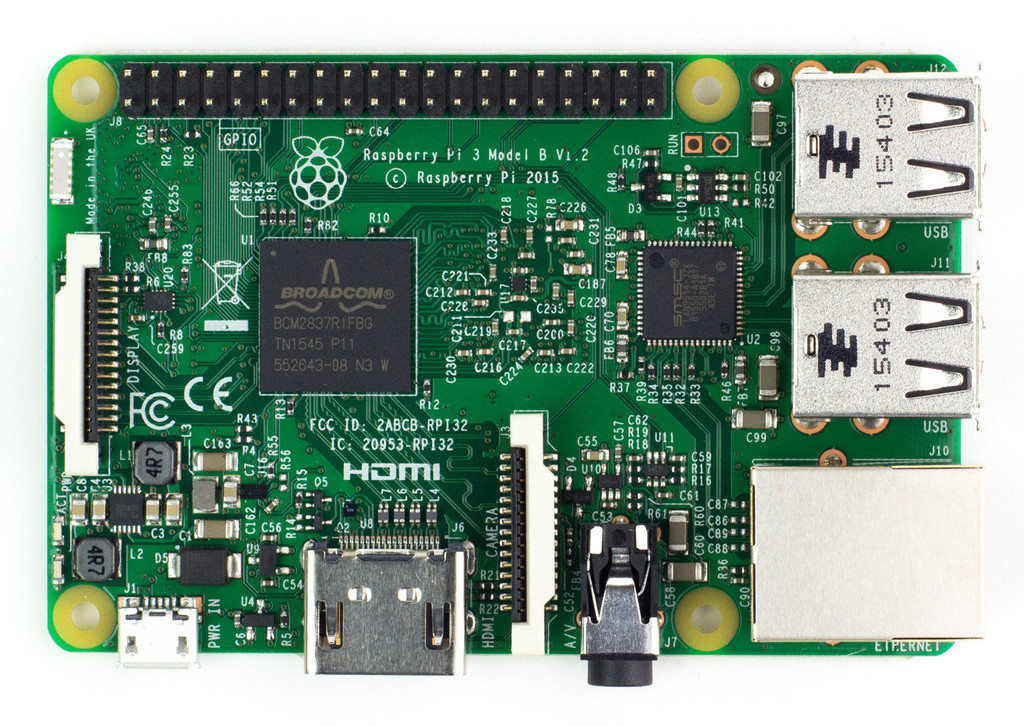
\includegraphics[width=0.5\linewidth]{\figures/photo_raspberry_pi_3.jpg}
    \decoRule
    \caption[
    Raspberry-Pi 3 B]{
    Raspberry-Pi 3 B}
    \label{fig:Raspberry-Pi 3 B}
    \end{figure}

\vspace{1cm}

La caméra utilisée sera celle fournie avec la Raspberry-Pi, à savoir le module Raspicam v2.1 intégrant une caméra IMX219 de $8Mpx$. L'écran sera choisi le moment venu s'il est intégré.

\subsection{Résumé des exigences}

\begin{figure}[H]
	\centering
    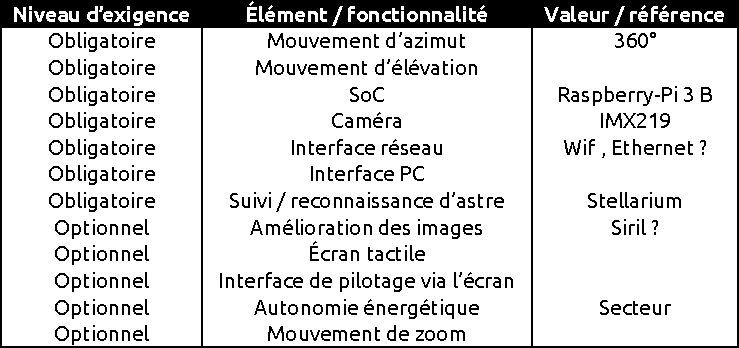
\includegraphics[width=0.7\linewidth]{\figures/tab_exigences.pdf}
    \decoRule
    \caption[
    Tableau récapitulatif des exigences du projet]{
    Tableau récapitulatif des exigences du projet}
    \label{fig:Tableau récapitulatif des exigences du projet}
	\end{figure}

